\begin{titlepage}
		\begin{center}
		\textbf{\Large Future Circular Collider}\\
        \vspace{0.5cm}
        \textbf{\LARGE Feasibility Study Report}\\
        \vspace{8 cm}
         \textbf{\Huge Volume 1}\\
        \vspace{1cm}
        \textbf{\Huge Physics, Experiments, Detectors}\\
        \vspace{3 cm}
        \textbf{ \today } \\
        \vspace*{\fill}
Submitted to the European Physics Journal ST, a joint publication of EDP Sciences,\\Springer Science+Business Media, and the Società Italiana di Fisica.
        \end{center}
\end{titlepage}

\section*{Note from the Editors}

\noindent One of the recommendations of the 2020 update of the European Strategy for Particle Physics was that “Europe, together with its international partners, should investigate the technical and financial feasibility of a future hadron collider at CERN with a centre-of-mass energy of at least 100 TeV and with an electron-positron Higgs and electroweak factory as a possible first stage.

\noindent In June 2021, the CERN Council launched the FCC Feasibility Study to be completed by 2025, in time for the next update of the European Strategy for Particle Physics. The study results are made publicly available through this FCC Feasibility Study Report, as input to the European Particle Physics Strategy update process, initiated by the CERN Council in March 2024. The studies presented in this FCC Feasibility Study Report do not imply any commitment by the CERN Member or Associate Member States to build the Future Circular Collider.

\noindent This report and the assumptions contained in it do not prejudge further territorial feasibility analysis by the Host States, France and Switzerland, as well as the outcome of their respective public debate and concertation processes, and future decisions of their relevant authorities.

\newpage

\section*{Acknowledgements}

We would like to thank the \textbf{International Steering Committee members:}\\


\vspace*{-3mm}


\begin{table}[!h]
	\small
	\centering
	\begin{tabular}{l}
		\toprule
		F.~Gianotti (Chair), CERN \\ 
		R.~Bello, CERN \\ 
		P.~Chomaz, CEA, France  \\ 
            M.~Cobal, INFN and University of Udine, Italy \\
		B.~Heinemann, DESY, Germany \\ 
		T.~Koseki, KEK, Japan \\ 
		M.~Lamont, CERN \\ 
		L.~Merminga, FNAL, United States \\ 
		J.~Mnich, CERN \\ 
		M.~Seidel, PSI and EPFL, Switzerland \\
		C.~Warakaulle, CERN \\
		\bottomrule
	\end{tabular}
\end{table}

\noindent and the \textbf{Scientific Advisory Committee members:}\\
\vspace*{-2mm}

\begin{table}[!h]
	\centering
	\small
	\vspace*{-3mm}
	\begin{tabular}{l}
		\toprule
		A.~Parker (Chair), Cambridge University, UK \\ 
		R.~Bartolini, DESY, Germany \\  
		A.~Chabert, SFTRF, France \\ 
		H.~Ehrbar, Heinz Ehrbar Partners LLC, Switzerland \\ 
		B.~Gavela Legazpi, UAM Madrid, Spain \\
		G.~Hiller, TU Dortmund, Germany \\
        S.~Krishnagopal, FNAL, U.S. \\		
        P.~Križan, University of Ljubljana, Slovenia\\
        P.~Lebrun, ESI, France\\
        P.~McIntosh, STFC, ASTeC,  UKRI, UK\\ 
        M.~Minty, BNL, U.S. \\  
        R.~Tenchini, INFN Sezione di Pisa, Italy  \\  
\bottomrule 
	\end{tabular}
\end{table}

\noindent for their continued guidance and careful reviewing that helped to complete this report successfully.\\

\newpage

\begin{wrapfigure}[4]{l}[0cm]{2cm}
  \begin{center}
  \vspace{-0.5cm}
    
\includegraphics[width=2cm]{frontmatter/eu_emblem.jpg}
  \end{center}
\end{wrapfigure}

\noindent
The research carried out by the international FCC collaboration hosted by CERN, which led to this publication, has received funding from the European Union's Horizon 2020 research and innovation programme under the grant numbers 951754 (FCCIS), 654305 (EuroCirCol), 764879 (EASITrain), 730871 (ARIES), 777563 (RI-Paths), 101086276 (EAJADE), 101004730 (iFAST), 101131435 (iSAS), 101131850 (RF2.0) and from FP7 under grant number 312453 (EuCARD-2).

\vspace{1em}

\begin{wrapfigure}[4]{l}[0cm]{2cm}
  \begin{center}
  \vspace{-0.85cm}
    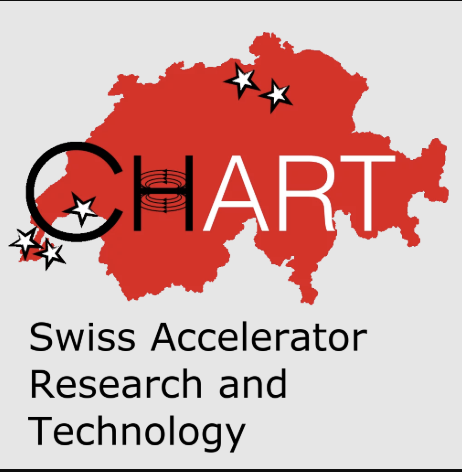
\includegraphics[width=2cm]{frontmatter/CHART-logo.png}
  \end{center}
\end{wrapfigure}

\noindent This work has also benefited from the support of CHART (Swiss Accelerator Research and Technology, founded in 2016 as an umbrella collaboration for accelerator research and technology activities. Present partners in CHART are CERN, PSI, EPFL, ETH-Zurich and the University of Geneva.

\vspace*{\fill}
\noindent\textbf{Trademark notice:} All trademarks appearing in this report are acknowledged as such.\\

\newpage

\noindent This report was edited with the Overleaf.com collaborative writing and publishing system. Typesetting and final print preparation was performed using pdf\TeX 3.14159265-2.6-1.40.17\\
\\
\noindent Copyright CERN for the benefit of the FCC collaboration 2025\\
Creative Commons Attribution 4.0\\
\\
Knowledge transfer is an integral part of CERN's mission.\\
CERN publishes this volume Open Access under the Creative Commons Attribution 4.0 licence.\\ (\mbox{\url{http://creativecommons.org/licenses/by/4.0/}}) in order to permit its wide dissemination and use.
The submission of a contribution to the CERN document server shall be deemed to constitute the contributor's agreement to this copyright and license statement. Contributors are requested to obtain any clearances that may be necessary for this purpose.

\bigskip
\noindent This volume is indexed in: CERN Document Server (CDS):

\smallskip
\noindent CERN-FCC-PHYS-2025-0002\\
\noindent 10.17181/CERN.9DKX.TDH9\\
\noindent \url{https://cds.cern.ch/record/2928193}\\

\bigskip
\noindent This report edition should be cited as:

\smallskip
\noindent Future Circular Collider Feasibility Study Report Volume 1: Physics, Experiments, Detector, preprint edition edited by \mbox{M.~Benedikt et al.}, CERN physics reports,\\
\mbox{CERN-FCC-PHYS-2025-0002},\mbox{DOI 10.17181/CERN.9DKX.TDH9}, Geneva, 2025.\\
\noindent Available online: \url{https://cds.cern.ch/record/2928193}
\clearpage


